\chapter{}
Diane looked around the pub for her friends. After a few minutes, she saw them at a table
near the corner. She hadn't seen any of them all summer, and this was their first get-together
of the new semester.

``Hey, Diane!'' one called out as she was spotted. She sat down with them. She quickly
caught up with the conversation. When the current topic had been exhausted, one of the girls
asked her:

``How's Monique doing?''

``I wouldn't know,'' Diane answered. ``When our apartment got hit, they offered to put us
up elsewhere, or just release us from our lease. Monique called me and said she wanted out, so I
got a different apartment.''

``Well, I would guess so, after what happened!''

``What do you mean?'' Diane asked. ``The storm? It was nasty and all, but I thought it was
kind of a crappy thing to do, ditching me as a roomie with no notice.''

``No- I mean because she got hurt so bad in the storm.'' The girl said.

``What are you talking about? I don't know anything about her getting hurt.''

``You're kidding! A wall fell on her in the storm. She broke a lot of bones. She's in a
huge body cast.''

``What?!'' Diane exclaimed.

``Yeah. She's in a cast from here down,'' the girl said, pointing to her midriff. ``You
haven't seen her since the storm?''

``No,'' Diane said. ``I talked to her on the phone. She said she didn't want to live there
anymore, and was going to pick up her things. I went back to the apartment a few days after the
storm to move my things out and she had already moved her stuff out. I haven't talked to her
since then.''

``Well, I can tell you this- she didn't come and get her stuff. Someone else must have
gotten it for her. Maybe it was her new boyfriend. She's really messed up. She says she's
healing nicely, but spending the whole summer lying on her back had to be terrible.''

\aside{Why wouldn't she tell me about it, if she'd gotten hurt so bad?''} Diane thought. The
conversation quickly changed, but thinking about Monique being injured bothered her. \aside{When
Monique told me she was moving out, I got pissed and yelled at her. Maybe I went off before she
got the chance to tell me, and she decided not to tell me at all. And why wouldn't she tell me
she had a boyfriend?} Something was very weird about all of this.

Monique's new cast certainly made daily life easier. Easier was, of course, relative. She
was still unable to move from the waist down, which was challenging enough. However, the
positioning of the new cast made classes easier, and the lighter weight made moving her around a
lot easier.

Monday morning had brought a new flurry of questions. She'd drawn a lot of attention from
friends and classmates when she'd started school in her huge cast, and now they wanted to know
about the new cast, and how her healing was going. We had brainstormed about this, and tried to
anticipate as many of the questions as possible. As I wheeled her into her first class, I
watched her handle them well.

``Hi Monique,'' asked a girl that I recognized from one of her classes later in the week.
``I like the purple! Are you still in one huge cast, or is it two, now?''

Monique lifted her t shirt just enough to show purple fiberglass on her midriff. ``Still
the one huge one,'' she sighed.

As we entered the classroom, another gal asked ``How is the healing going? When are you
going to be out of that thing?''

``The doctor says I'm healing well, but he still wants me in a cast. I go back in two weeks
for more x-rays; hopefully I can get out then.''

``At least you're not laying down in the new cast. That has to make things easier.''

``Almost everything,'' Monique said. ``Sleeping is difficult. I really only have two
choices- sitting up, or lying on my side. I'll get used to it.

Most of the questions were along those lines. After lunch, we had some time before classes
began, and we were in the courtyard talking when Megan, the nursing student came up and asked
some more pointed questions. Megan asked about the specific injuries that Monique had named when
she'd been asked about what landed her in such a big cast. Though we hadn't prepared for this,
Monique handled it well:

``The doctor says it looks like near complete healing in the long bone in my right leg, and
the ankle is coming along well, too. He said the pelvis and hip are also close. The left leg is
the farthest. Both bones in the left leg were broken in two places, and he said from the start
that it would be the slowest injury to heal.''

``So when do you go back and see him again?'' Megan asked.

``I go back a week from Friday.''

Megan concerned me. The questions she asked were very specific and the tone she took made
me wonder if she doubted Monique's story about the injuries. Considering that she was studying
nursing, the questions she asked made me uncomfortable. Monique, however, was a good actress,
and fielded the questions in a very convincing manner. Apparently, she was a very good actress,
because what Megan asked next put me more at ease:

``Monique, I know this has been a rough summer. I'm sure that getting hurt was terrible,
and that you had to deal with a lot of pain. I can sort of imagine how difficult it is living in
the cast, but I want to ask a favor. Sometime when you have the time, I'd love to sit down and
talk about the whole thing. I think it might help with my studies, and it will definitely help
when I'm out working. Would you mind doing that?''

``No, of course, not,'' Monique answered.

They compared schedules, and decided that Tuesday evening would be the best time for both
of them.

After the flurry of questions on Monday, things settled down. Classes were getting into the
meat of the work, and everyone (including Monique) was getting into a routine and concentrating
on getting to work. So, while she was still drawing attention, she wasn't drawing as much.

Our daily life was pretty smooth by this point, as well. Monique had been in the double hip
spica for almost two weeks, and we'd found out how to cope with it when we weren't openly
enjoying it. The new cast had caused a few adjustments in the proper way to attach the harness
for lifting her in and out of the truck. Getting her into and out of the wheelchair was much
easier with the lighter cast, and we quickly discovered a couple of positions for making love
with her in the new cast. They were odd positions, but the situation dictated creativity, and we
met the challenge.

It was nice having Monique home in the evening every night. She'd planned to take the first
two weeks off from work while she settled in to her new routine. When our adventure had
blossomed into actually faking serious injuries for a long period of time, she'd called her
manager to ask for an extended leave for medical reasons. Her request was not taken well, and
when her manager had questioned her, she was a bit vague about the nature of her reason. He told
her that unless she had proper FMLA paperwork, he did not have to hold her job for her. He also
told her that since he would have to hire someone to cover for her while she was out, she
couldn't expect to get as many hours once she returned. His attitude had struck Monique the
wrong way, and she resigned her position outright, with a promise to me that she'd find another
job once the cast charade was over.

During our evenings at home, we worked on the details for the upcoming trips we had
planned. The car show in Illinois was coming up quickly. Driving the Shelby to the show would be
great, but we couldn't enter it, since the show was for cars from the 1965 model year and older.
We decided that we'd leave it at home for security reasons. We would be staying a couple of
nights, and parking lot security at hotels is notoriously terrible.

We also spent time looking at different things to see and do in the Smoky Mountains.
Clearly, the Gatlinburg and Pigeon Forge areas were heavily built up with things to attract
tourists. That sort of thing held very little appeal for either of us, but the natural beauty of
the area was definitely something we both looked forward to. There were hiking trails that we
wanted very much to try, and some historic sites we wanted very much to visit. And, who knows,
we might try a touristy thing or two, also.

We also had a lengthy conversation about her continuing ``recovery.'' On Wednesday I
approached Monique with a question.

``Monique, what do you think about cam walkers?'' I asked.

She scrunched her nose up a bit. ``They're kind of a cheat. A cast that should have been.''

``True,'' I said. ``But it's also a way that someone who isn't really injured could keep up
the appearance, and still be free when in private.''

We discussed what the exact course of her ``treatment'' would be once she was out of the
hip spica. She still had a week and a half to go before we had to make the decision, but it
wasn't too soon to be thinking about it. From the story that she'd been telling, as well as from
our plans, the hip spica had to go after next weekend. After that, she could have her right leg
in a long or short cast, a cam walker, or completely free. She'd indicated that the left leg was
the slower healing one, so leaving it completely free wasn't an option, but everything else was.
We didn't reach any definite decision, but we agreed that I would order two cam walkers so that
we would have them if we wanted to use them.

Thursday evening, I carefully photographed the few signatures that Monique had collected on
the new cast. She'd remembered the types of pens that had been used, and I made a quick trip to
get what I needed to reproduce them.

Friday, when she was done with school for the day, we went home, took a few final photos,
and cut her out of the cast. As we did the week before, I cut the cast off in two halves, which
we saved, as usual.

\begin{thought}
Coming out of the cast this time was a bit more difficult than it had been last week.
Monique noticed that there was more stiffness this time than last week, and that her legs felt
weaker than they had when they'd taken the first hip spica off. She did her best to hide this
fact from Quinn, and wasn't sure if she had been able to pull it off or not.

The soak in a hot bath helped loosen things up, and quickly, she was on the elliptical and
rowing machines, working the muscles that had sat mostly unused through the week. Clearly, the
second week of immobility had taken more of a toll than the first.

Over the past couple of weeks, she had planned to try to convince Quinn to let her wear two
long leg casts after the spica came off. With the way things were aching right now, she began to
consider going a bit smaller.
\end{thought}

Sunday night, we once again retreated to the cast room as the sun went down. Because I'd
left all of the attachments in the same adjustment that they'd been in when we made the previous
cast, the next one was a virtual duplicate of it. If someone had studied pictures, they might
notice a different wrapping pattern to the fiberglass, but without the previous one to compare
to, there was no way to tell that they were different casts. Once I'd duplicated the few
signatures she'd collected, we had no doubts that it would be totally convincing.

Monique looked so beautiful in the cast, but my feelings were conflicted. I was concerned
about the extended immobility. She hadn't moved as well during her time out of the cast these
past two days as she had the previous weekend. She hadn't complained, nor even mentioned it, but
I noticed nonetheless. I reminded myself that there was only one more week of this part of the
ruse, and then things would be better.

\begin{thought}
Sitting there, wearing nothing but her cast and underwear, Monique watched as Quinn
sketched her in the new cast. It never got old, watching him work. As he was drawing, she was
already doing the isometric exercises, with the cast as the resistance. Though the stiffness and
weakness had been a bit more pronounced this weekend, she had one more week to go in the double
hip spica, and she planned to enjoy every minute of it. It would start with some casted
lovemaking, just as soon as the drawing was finished.
\end{thought}

\newpage
\begin{center}
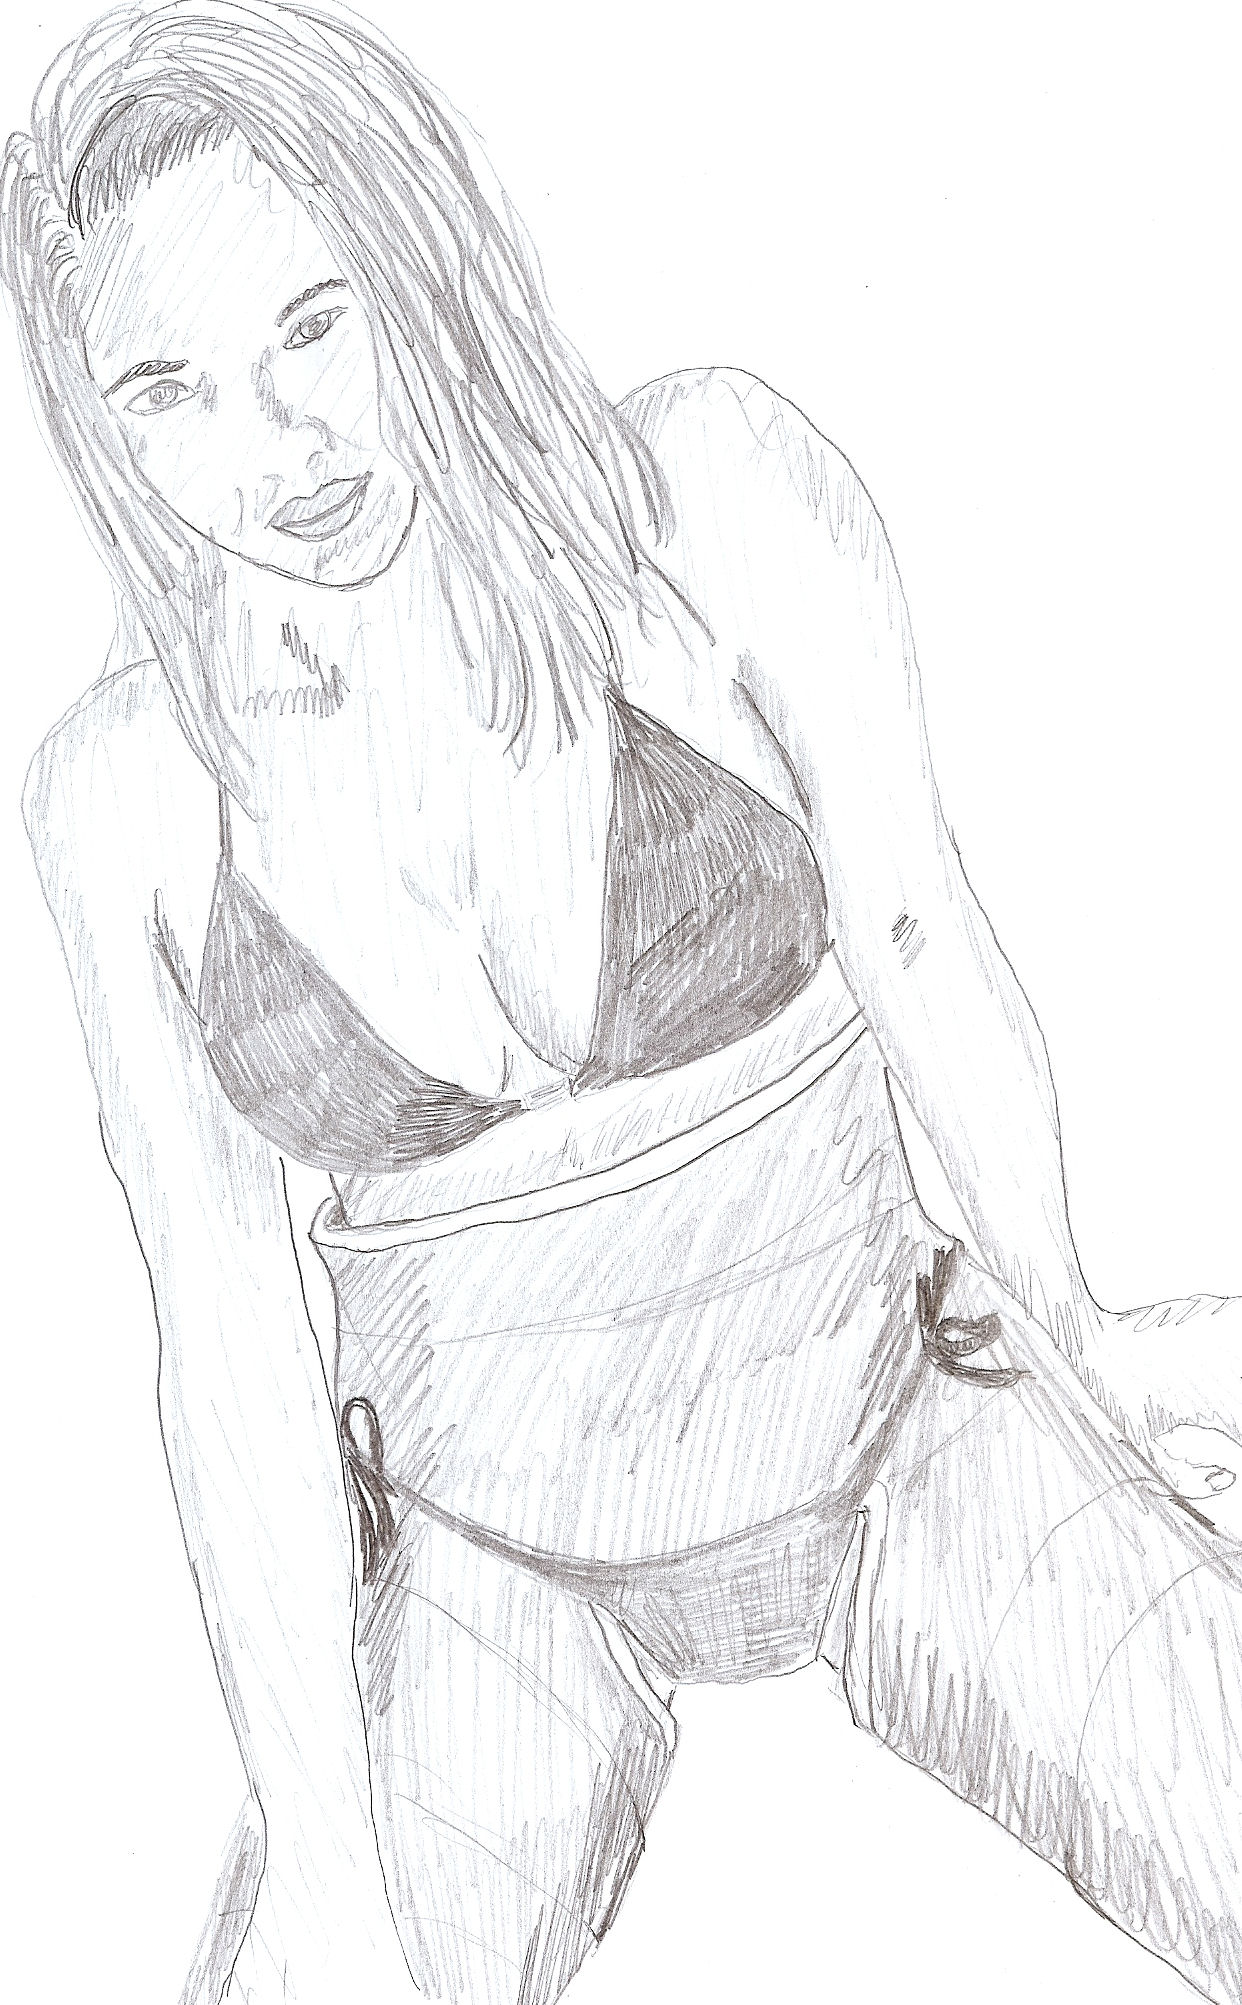
\includegraphics[height=\textheight]{images/kicks48.jpg}
\end{center}
